\subsection{旋转构建垫片的三维模型}
\begin{procedure}
\item 通过建模中的【旋转】操作产生三个圆柱。

旋转产生$\phi 104$直径圆柱。
\begin{lstlisting}
|命令: REVOLVE|
|当前线框密度:  ISOLINES=4,闭合轮廓创建模式 = 实体|
|选择要旋转的对象或 [模式(MO)]: 找到 1 个|
|选择要旋转的对象或 [模式(MO)]:|
|指定轴起点或根据以下选项之一定义轴 [对象(O)/X/Y/Z] $<$对象$>$:|
|指定轴端点:|
|指定旋转角度或 [起点角度(ST)/反转(R)/表达式(EX)] $<360>$:|
\end{lstlisting}
旋转产生$\phi 53$直径圆柱
\begin{lstlisting}
|命令:  REVOLVE|
|当前线框密度:  ISOLINES=4,闭合轮廓创建模式 = 实体|
|选择要旋转的对象或 [模式(MO)]: 找到 1 个|
|选择要旋转的对象或 [模式(MO)]:|
|指定轴起点或根据以下选项之一定义轴 [对象(O)/X/Y/Z] $<$对象$>$:|
|指定轴端点:|
|指定旋转角度或 [起点角度(ST)/反转(R)/表达式(EX)]$ <360>$:|
\end{lstlisting}
旋转产生$\phi 8$直径圆柱
\begin{lstlisting}
|命令:  REVOLVE|
|当前线框密度:  ISOLINES=4,闭合轮廓创建模式 = 实体|
|选择要旋转的对象或 [模式(MO)]: 找到 1 个|
|选择要旋转的对象或 [模式(MO)]:|
|指定轴起点或根据以下选项之一定义轴 [对象(O)/X/Y/Z] $<$对象$>$:|
|指定轴端点:|
|指定旋转角度或 [起点角度(ST)/反转(R)/表达式(EX)]$ <360>$:|
\end{lstlisting}
\item 关闭“中心线”图层。
\item 切换视图为西南等轴测图。

切换后的结果如图\ref{fig:3darray}所示。
\begin{figure}[htbp]
\centering
\subfloat[]{\label{fig:3darray}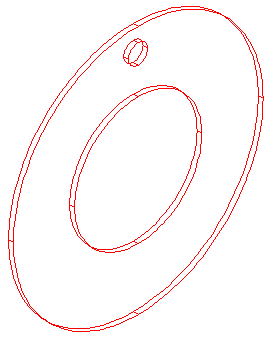
\includegraphics[scale=0.5]{3darray.png}}\hspace{30pt}
\subfloat[]{\label{fig:3darrayselect}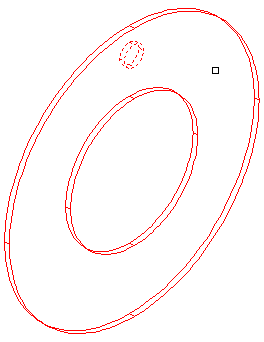
\includegraphics[scale=0.5]{3darrayselect.png}}\hspace{30pt}
\subfloat[]{\label{fig:3darrayresult}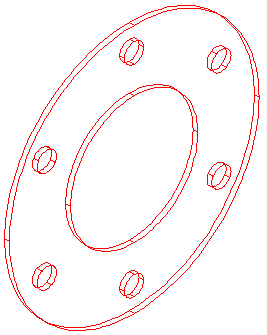
\includegraphics[scale=0.5]{3darrayresult.png}}
\caption{三维阵列过程}
\end{figure}
\item 阵列产生圆柱体。

用【三维阵列】命令阵列$\diameter 8$的圆柱,其结果如图\ref{fig:3darrayresult}所示。

启动【三维阵列】命令的方法有:
\begin{itemize}
\item 键盘输入3DARRAY\index{3darray}。
\item 【修改】$\rightarrow$【三维操作】$\rightarrow$【三维阵列】。
\item 【建模】$\triangleright$【三维阵列】图标
\includegraphics[scale=0.6]{3darraytool.png}。
\end{itemize}

按图\ref{fig:3darrayselect}所示的选择$\diameter 8$圆柱作为三维阵列对象
\begin{lstlisting}
|命令: 3darray|
|选择对象: 找到 1 个|
|选择对象:|
\end{lstlisting}
指定三维阵列的类型为环形。
\begin{lstlisting}
|输入阵列类型 [矩形(R)/环形(P)]$<$矩形$>$:p|
\end{lstlisting}
指定三维阵列项目的数量为6个。
\begin{lstlisting}
|输入阵列中的项目数目: 6|
\end{lstlisting}
指定三维阵列项目的填充角度为360度。
\begin{lstlisting}
|指定要填充的角度 (+=逆时针, -=顺时针)$ <360>$:|
\end{lstlisting}
指定是否旋转阵列对象。
\begin{lstlisting}
|旋转阵列对象? [是(Y)/否(N)] $<Y>$:|
\end{lstlisting}
选择$\diameter 104$圆柱的后底圆圆心为阵列中心线第一端点。
\begin{lstlisting}
|指定阵列的中心点:|
\end{lstlisting}
选择$\diameter 104$圆柱的前顶圆圆心为阵列中心线第二端点。
\begin{lstlisting}
|指定旋转轴上的第二点:|
\end{lstlisting}
\item 用差集操作完成垫片的三维建模操作。
\begin{lstlisting}
|命令: subtract |
|选择要从中减去的实体、曲面和面域...|
|选择对象: 找到 1 个|
|选择对象:  选择要减去的实体、曲面和面域...|
|选择对象: 找到 1 个|
|选择对象: 找到 1 个,总计 2 个|
|选择对象: 找到 1 个,总计 3 个|
|选择对象: 找到 1 个,总计 4 个|
|选择对象: 找到 1 个,总计 5 个|
|选择对象: 找到 1 个,总计 6 个|
|选择对象: 找到 1 个,总计 7 个|
|选择对象:|
\end{lstlisting}
\item 设置视觉样式为真实,其结果如图\ref{fig:dianpiansolid}所示。设置方法为:点击【视图】菜单中【视觉样式】子菜单中的【真实】项。
\item 将垫片模型保存为“调压阀垫片立体图.dwg”。
\end{procedure}
\endinput